\documentclass[12pt,oneside]{sigmasthesis}

% The goal is to update Ross's template and make it helpful for all SIGMAS members.
% This template uses an updated version of Ross's uvicthesis document class, now called sigmasthesis.
% Place the class file in the same folder as the document file.

% Original template by Ross Churchley, circa 2011 or so
% Updated by Joseph Horan, Spring 2020

% Use 12pt font (people will thank you for not using a smaller font).
% The oneside option is passed to the underlying book class; it horizontally centers the pages, instead of forcing a book-style page turn. Page-numbering is adjusted to be symmetric in the class.

%--------------------------------------------------------------------------------------%
%								YOUR INFORMATION										
%--------------------------------------------------------------------------------------%

\title{Tight Bounds on 3-Neighbor Bootstrap Percolation}			% Title of your thesis/dissertation
\type{Thesis}				% "Thesis" (MSc) or "Dissertation" (PhD)
\author{Abel Emanuel Romer}			% Your (full) name!
\authordetails{B.A.Sc., Quest University Canada, 2017}	% Past degrees in reverse order, eg. "MSc, University of Victoria, 2015 \\ BMath, University of Waterloo, 2013"
\degree{Master of Science}			% Title of your degree: "Master of Science", "Doctor of Philosophy"; be sure to spell it correctly!
\department{Department of Mathematics and Statistics}	% This is your home department, unless you are dual-department, in which case you should write "Departments of Mathematics and Statistics and Geography" or similar. If you are Interdisciplinary, you must change the class file: in the maketitlepage command, you must change "in the" to "in", then back here you write "Interdisciplinary Studies".
\date{2022}				% The year!

%--------------------------------------------------------------------------------------%
%								YOUR SUPERVISORY COMMITTEE										
%--------------------------------------------------------------------------------------%
\panel{% This list should include everyone on your supervisory committee; do NOT include your external examiner (they are not a member of your supervisory committee). For non-UVic committee members, list external affiliation.
\panelist{Dr. Peter Dukes}{Co-Supervisor}{Department of Mathematics and Statistics} % {Dr. First Last}{(Co-)Supervisor}{Department of ...}
\panelist{Dr. Jonathan Noel}{Co-Supervisor}{Department of Mathematics and Statistics} % {Dr. First2 Last2}{Co-Supervisor or Departmental Member}{Department of ...}
%\panelist{ }{ }{ } % {Dr. First3 Last3}{Outside Member}{Department of ...}
%\panelist{ }{ }{ } % {Dr. First4 Last4}{Additional Member}{Department of ..., University of ...}
% and so on.
}

%--------------------------------------------------------------------------------------%
%								YOUR OWN PACKAGES AND CUSTOMIZATIONS
%--------------------------------------------------------------------------------------%
% Here's some useful packages to start out with, but feel free to delete them and replace
% them with your own!
\usepackage{amsmath, amsthm, amssymb}
\usepackage{graphicx}
\usepackage{tikz}
\usepackage{booktabs} % See the package documentation for guidelines on formal tables: https://ctan.org/pkg/booktabs
\usepackage{verbatim} % Used to typeset, for example, code snippets or pseudo-code for algorithms.
\usepackage{dsfont} % Extra fontset for helpful mathematics symbols, e.g. \mathds{1}
\usepackage{etoolbox} % Used to allow boolean variables for use in the title page

% The underlying document class ------ loads the following packages: setspace, titlesec, fancyhdr, textcase, tocloft.

% Put your custom macros for commands. These are just some suggested ones.

\newcommand{\R}{\mathbb{R}}
\newcommand{\Q}{\mathbb{Q}}
\newcommand{\C}{\mathbb{C}}
\newcommand{\N}{\mathbb{N}}
\newcommand{\Z}{\mathbb{Z}}
\newcommand{\T}{\mathbb{T}}

\newcommand{\cA}{\mathcal{A}}
\newcommand{\cB}{\mathcal{B}}
\newcommand{\cD}{\mathcal{D}}
\newcommand{\cP}{\mathcal{P}}
\newcommand{\cM}{\mathcal{M}}

\newcommand{\abs}[1]{\left\lvert #1 \right\rvert}
\newcommand{\norm}[1]{\left\lVert #1 \right\rVert}
\newcommand{\set}[2]{\left\{#1 \ : \ #2\right\}}
\newcommand{\conv}[1]{\underset{#1}\longrightarrow}

% A custom restriction command, indicate that a function is being restricted to a subset of its domain.

\newcommand\restr[2]{{% we make the whole thing an ordinary symbol
  \left.\kern-\nulldelimiterspace % automatically resize the bar with \right
  #1 % the function
  \vphantom{\big|} % pretend it's a little taller at normal size
  \right|_{#2} % this is the delimiter
  }}

% Custom math operators (analogous to \lim, \sup, etc).

\DeclareMathOperator{\id}{id}
\DeclareMathOperator{\subspan}{span}
\DeclareMathOperator{\sgn}{sgn}

% Custom List of ... commands. See the tocloft package documentation for more details.

% Any new lists of --- (for example, a List of Abbreviations, a List of Terms, etc) can be defined using the functionality in the package tocloft. This allows all lists in the preliminary pages to share the same formatting (as per UVic guidelines). 
% The following is a sample that you could use to include a list of abbreviations in the document.
% You could also create a glossary in a similar way.

%\newlistof[section]{abbrevs}{abr}{List of Abbreviations}
%\newcommand{\abbrevs}[2]{%   The command takes in two parameters: a phrase and its abbreviation.
%	\refstepcounter{abbrevs}#1 (#2)% This line associates a number with the entry and typesets something there.
%	\addcontentsline{abr}{abbrevs}{\numberline{}#2 - #1}}	% This line adds a line to the List of Abbreviations.

%--------------------------------------------------------------------------------------%
%								THEOREM ENVIRONMENTS
%--------------------------------------------------------------------------------------%

% Again, feel free to replace these with whatever is best for you! Look at the amsthm package documentation for more info.

% Tips for theorem numbering: While it's up to you, you might wish to try a system that makes it easiest to find results, and if two systems are equally easy to use, then use the simpler of the two. Generally you will have chapters or sections in your document, so numbering at least 1.1, 1.2, 2.1, 2.2, 2.3, ... might be good; if you also have subsections, maybe you could do 1.1.1, 1.1.2, 1.2.1, 1.2,2, etc, together with numbered subsections. You might also do unnumbered subsections and use only section numbering, if the subsections tend to be short.

% These environments are theorem-like; they have bold labels and italicized text. 

\newtheorem{thm}{Theorem}[chapter] % Numbering is impacted by [chapter]; could do [section] or [subsection] also.
\newtheorem{lem}[thm]{Lemma} % The [thm] argument says to number Lemma in sequence with Theorem.
\newtheorem{prop}[thm]{Proposition}
\newtheorem{cor}[thm]{Corollary}

% These environments are unnumbered and will not count toward the numbering.

\newtheorem*{question}{Question}
\newtheorem*{answer}{Answer}
\newtheorem*{conjecture}{Conjecture}

% These environments are definitions; they have a different style (bold label, standard font).

\theoremstyle{definition}
\newtheorem{defn}[thm]{Definition} % These definitions are also numbered in sequence with Theorem.
\newtheorem{eg}[thm]{Example}
\newtheorem{rem}[thm]{Remark}


%--------------------------------------------------------------------------------------%
%								FRONTMATTER										
%--------------------------------------------------------------------------------------%
\begin{document}
\frontmatter 	% From the class file, sets small spacing and roman numeral page numbering

\newbool{terr-ack}
\booltrue{terr-ack} % Uncomment to include the standard UVic Territory Acknowledgement in your title page at the bottom; leave commented to leave it out.
\maketitle{terr-ack}	% Typesets the title page (as redefined by the class file). 

\makecommittee	% Typesets the committee page (as defined by the class file).

\begin{abstract}
% Here is where the abstract goes; it gets typeset on its own page. No required length, but recommended ~250 words.
\end{abstract}

\newpage\addtoToC{Table of Contents}\tableofcontents % Typesets the Table of Contents; LaTeX handles this. Here, because I wrote ``Table of Contents'' as the name of the entry, then I should go into the class file and change \contentsname to whatever I just put, so that the name and the header match. Default for \contentsname is ``Contents''.
\newpage\addtoToC{List of Tables}\listoftables % Uncomment to add a list of Tables to the Table of Contents; required if you have any tables.
\newpage\addtoToC{List of Figures}\listoffigures % Uncomment to add a list of Figures to the Table of Contents; required if you have any figures.
%\newpage\addtoToC{...}\listof... % Any other custom lists, defined as above.

\begin{acknowledgements} 
	\vskip 2\baselineskip
	\noindent % If you have acknowledgements, place them here. If you do not, comment out the whole begin-end block. These need to go before the Dedication. Depending on your choice, you may wish to indent or not indent the whole thing.
\end{acknowledgements}

\begin{dedication} 
	\vskip 2\baselineskip
	\noindent % If you have dedications, place them here. If you do not, comment out the whole begin-end block.
\end{dedication}
%--------------------------------------------------------------------------------------%
%								MAIN CONTENT										
%--------------------------------------------------------------------------------------%
\mainmatter % Switches spacing back to default and arabic page numbers (and implements a page break).

% Start writing here! This is the main body of the document. Some folks like to type everything here, in one document; you could also use an \input (verbatim inclusion of a file into this one) or \include (adds page breaks, etc; you would \include a chapter file, for example, which would allow you to \includeonly some of your chapters when compiling) to fill in your content.

\chapter{Introduction} % Use \chapter*{} if you don't want the chapter numbered; similarly for sub/sections.

\section{Problem Overview}

\section{Literature Review}

\section{Outline of ...}

\chapter{A Tight Bound on Grids of Size $\geq$ 7}

\section{Introduction and Definitions}
Let the ordered tuple $(a,b,c)$ represent the $a \times b \times c$ grid $G$ where $a \geq b \geq c$. We refer to $c$ as the ``thickness" of $G$. For example, the tuple $(5,3,3)$ represents a $5 \times 3 \times 3$ grid of thickness 3. We refer to a tuple as ``divisible", or a ``divisibility case", if and only if $ab+bc+ca \equiv 0 \pmod 3$. Observe that the divisibility cases are precisely those grids with integral lower bounds. The divisibility cases of thicknesses belonging to the three residue classes modulo 3 are illustrated in \{Figure something\}.

In the following lemmas, we use the notation $(a,b,c)+(x,y,z) = (a+x, b+y, c+z)$ to represent respective increases of $x$, $y$, and $z$ to the side lengths $a$, $b$, and $c$ of $G$. We note the following: 
\begin{rem}
By applying the recursion, $(a,b,c)+(x,y,z)$ percolates at the lower bound when either:
\begin{enumerate}
\item $(a,b,c), (a,y,z), (x,b,z), (x,y,c)$ all percolate at the lower bound, or;
\item $(x,y,z), (x,b,c), (a,y,c), (a,b,z)$ all percolate at the lower bound.
\end{enumerate}
\end{rem}

We shall call a thickness ``complete" if it can be shown that all divisibility cases in that thickness percolate at the lower bound. In this section, we demonstrate that thickness 5, thickness 6 and thickness 7 are all complete. As these belong to the residue classes 2, 0, and 1 modulo 3, respectively, we then use a recursive construction to show that all larger grids are also complete. 

\section{Completeness of Thickness 5}
Leveraging \{lemmas from earlier chapters yet to be written\}, we show that all divisibility cases in thickness 5 percolate at the lower bound. 

\begin{lem}
Thickness 5 is complete.
\end{lem}

\begin{proof}
Let $(a,b,2)$ represent an arbitrary (divisible) grid of thickness 2, and let $x = a \pmod 6$ and $y = b \pmod 6$. By \{some as of yet unwritten construction\}, we have that $(a,b,2)$ percolates at the lower bound for all $x,y \in \{0,2,3,5\}$, where $x \neq y$. We consider two constructions: $(a,b,2) + (6,3,3)$ and $(a,b,2) + (6,6,3)$. 

By item (1) of the remark, in order to show that $(a,b,2) + (6,3,3)$ percolates at the lower bound, it is sufficient to show that $(a,b,2), (a,3,3), (6,b,3), (6,3,2)$ all percolate at the bound. By \{more unwritten constructions\}, this is true for all $x,y \in \{0,2,3,5\}$, where $x \neq y$ and at least one of $\{a,b\} > 2$. (Note that if $a=2$, one of the tuples is $(2,3,3)$, which does not percolate at the lower bound; we accommodate for this by re-writing $(a,b,2) + (6,3,3)$ as $(a,b,2) + (3,6,3)$.) The resulting tuple $(a', b', 5)$ is a grid of thickness 5, with $a'$ and $b'$ in the same residue class modulo $6$, and at least one of $\{a',b'\} \geq 9$. From \{some figure representing the divisibility cases of thickness 5\}, we see that the lower bound on $a'$ and $b'$ omits the following three grids: $(5,5,5), (6,6,5)$ and $(8,8,5)$. 

Applying an analogous argument to $(a,b,2) + (6,6,3)$, we must demonstrate that $(a,b,2), (a,6,3), (6,b,3), (6,6,2)$ all percolate at the lower bound. By \{some other constructions\}, we again find that this holds for all $x,y \in \{0,2,3,5\}$, where $x \neq y$ and $a,b > 1$. This gives all thickness 5 tuples $(a',b', 5)$ with $a'$ and $b'$ in different residue classes modulo $6$, where $a',b' \geq 8$. 

SOMETHING IS DIFFERENT

\begin{figure}[]
\centering
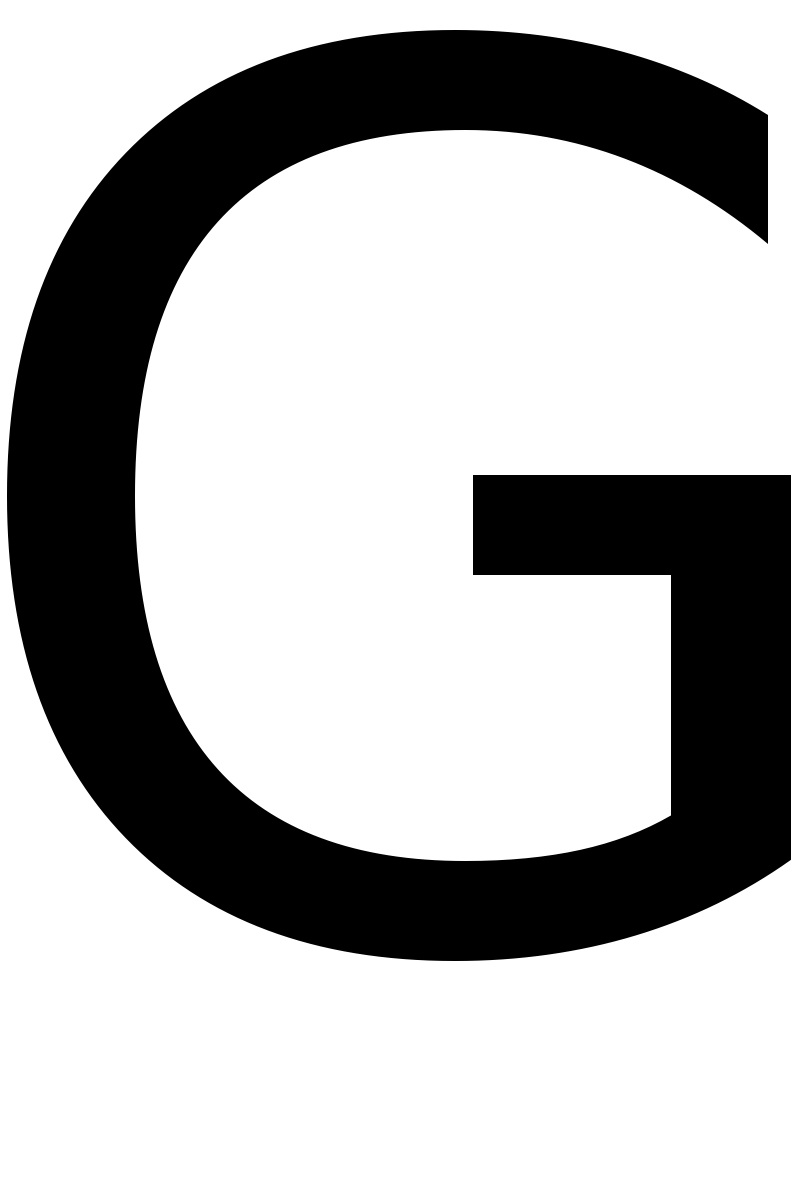
\includegraphics[height=1in]{figures/3/test.png}
\end{figure}

\end{proof}

\subsection{Intuition and Statement}

\subsection{Proof}

\chapter{Chapter on the Next Thing}

% etc.


%--------------------------------------------------------------------------------------%
%								BIBLIOGRAPHY										
%--------------------------------------------------------------------------------------%

\backmatter % Makes the Bibliography an unnumbered section (and implements appropriate page breaks).
	\addtoToC{Bibliography}
	\bibliographystyle{abbrv} % Choose the style that you want to use (or your supervisor wants you to use).
	\bibliography{} % Use your bibtex file. 

\end{document}
